\documentclass{article}
\usepackage[utf8]{inputenc}
\usepackage{graphicx}
\usepackage{amsmath}

\usepackage{amsthm}
\newtheorem*{remark}{Remark}
\theoremstyle{definition}
\newtheorem{definition}{Definition}[section]

\theoremstyle{remark}

\title{Lecture 39 - Sourced Gravitational Waves Continued}
\author{Alex Leviyev}
\date{May 2020}

\begin{document}

\maketitle

\section{Gravitational waves from two body problem}
In this first section we are going to look at gravitational waves from a circular binary using Newtonian mechanics (assuming $v << c$). With this framework we will calculate the second moment of the mass distribution (the quadrupole moment) $I_{ij}$, and ultimately arrive at the metric perturbations in the TT gauge (this will represent the gravitational waves).

\begin{figure}
    \centering
    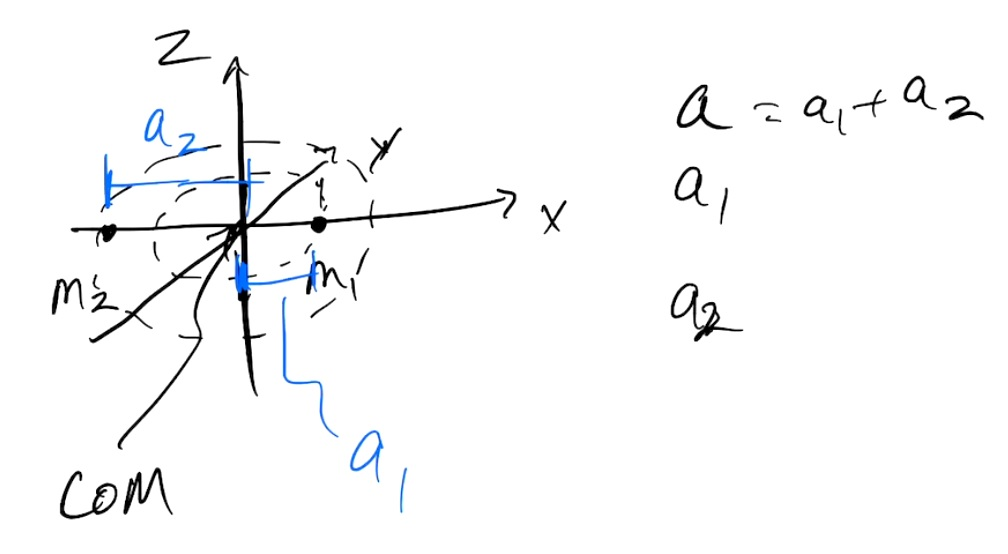
\includegraphics{figures/binary diagram.jpg}
    \caption{Binary system schematic. Masses $m_1$ and $m_2$ perform circular orbits around the center of mass. $a$ is the separation between the two masses, and $a_1$ and $a_2$ are the position vectors to the respective masses from the center of mass}
    \label{fig:binary}
\end{figure}

To solve this two-body problem we employ the two-body formalism from classical mechanics. This allows us to transform the two body problem (where two objects are moving) to an equivalent problem where only one object is moving. We will not go in depth into the formalism, bet we will setup the solution and state relevant results. The setup is as follows (Figure \ref{fig:binary}). Let $\mu = \frac{m_1 m_2}{m}$ where $m = m_1 + m_2$. Then the trajectories remain in the z axis, and are given by:


$$
x_1 = a_1 \cos \Omega t \: \: \: y_1 = a_1 \sin \Omega t \: \: \: z_1 = 0
$$

$$
x_2 = -a_2 \cos \Omega t \: \: \: y_2 = -a_2 \sin \Omega t \: \: \: z_2 = 0
$$

Now that we have the trajectories, recall that the second mass moment collapses to a sum over the individual particles. Explicitly:
\begin{equation}
I_{ij} = \sum_{a=1}^2 m_a x_i^a x_j^a
\end{equation}\label{eq:mass_moment}

Plugging in the trajectories into Equation \ref{eq:mass_moment},

$$
I_{11} = \mu a^2 \cos ^2 \Omega t
$$

$$
I_{12} = \mu a^2 \sin ^2 \Omega t
$$

The rest of the components vanish! Now we need second time derivative of these quantities to get the trace reversed perturbation.
$$
\ddot{I_{xx}} = - \frac{\mu a^2}{2} 4 \Omega^2 \cos 2 \Omega t 
$$

\begin{remark}
Recall that Keplers third law is $m = \Omega^2 a^3$ with $G = 1$. We will use this to simplify our expressions.
\end{remark}
\begin{remark}
$m \Omega$ is a dimensionless quantity, since m is measured in length, and frequency is inverse time, recalling that time has units of length as well. This is a useful grouping to make.
\end{remark}

Using Keplers law, we can find that $a^2 = (\frac{m}{\Omega ^2})^{2/3}$
With these results, we see 

$$
\ddot{I_{xx}} = - 2 \mu (m \Omega)^{2/3} \cos 2 \Omega t = - \ddot{I_{yy}} 
$$

Note how this turns out to make $\ddot{I_{ij}}$ traceless. 

$$
\ddot{I_{xy}} = - 2 \mu (m \Omega)^{2/3} \sin 2 \Omega t 
$$



$$
h_{ij} = \frac{2\ddot{I_{ij}}(t-r)}{r}
$$

There is a hidden angular dependence here! We now need to apply the TT projection.

$$
P_i^a = \delta_i^a - n_i n^a
$$

\begin{equation}
h_{ij}^{TT} = (P_i^a P_j^b - 0.5 P_{ij} P^{ab}) h_{ab}
\end{equation}\label{eq:tt_metric}

Note that we will get different results when we project onto different axes. These projections are related to different observing directions of this binary. Applying this projection operator onto the z axis gives:
$$
h_{ij}^{TT} = -4 \mu / r \: (m \Omega)^{2/3}
\begin{bmatrix}
- \cos 2 \Omega t_r & - \sin 2 \Omega t_r & 0\\
 - \sin 2 \Omega t_r &  \cos 2 \Omega t_r  & 0\\
 0 & 0 & 0
\end{bmatrix}
$$
From this we can read of the $h_+$ and $h_\times$ polarizations:

$$
h_+ = -4 \mu / r \: (m \Omega)^{2/3} \cos 2 \Omega t_r
$$

$$
h_\times = -4 \mu / r \: (m \Omega)^{2/3}  \sin 2 \Omega t_r
$$

\begin{remark}
We see that for a circular binary an observer on the z-axis sees two differently polarized waves. In particular, these waves are shifted $\frac{\pi}{2}$ rad from each other. This is called "circular polarization".
\end{remark}

How would things be different if the observer is on the x axis? Well, lets repeat the process.


$$
P_i^a = 
\begin{bmatrix}
0 & 0 & 0\\
0 & 1 & 0\\
0 & 0 & 1
\end{bmatrix}
$$.

Recalculating the projection for the x-axis. Using Equation \ref{eq:tt_metric}, we get:

$$
h_+ = - \frac{2 \mu}{r}  (m \Omega)^{2/3} \cos 2 \Omega t_r 
$$

$$
h_\times = 0
$$

\begin{remark}
Note that this makes sense, because it looks like the system is oscillating horizontally. Note how the answer indeed depends on from where we observe this binary!
\end{remark}

Lets look at the projection operator in general now. In general:

\begin{figure}
    \centering
    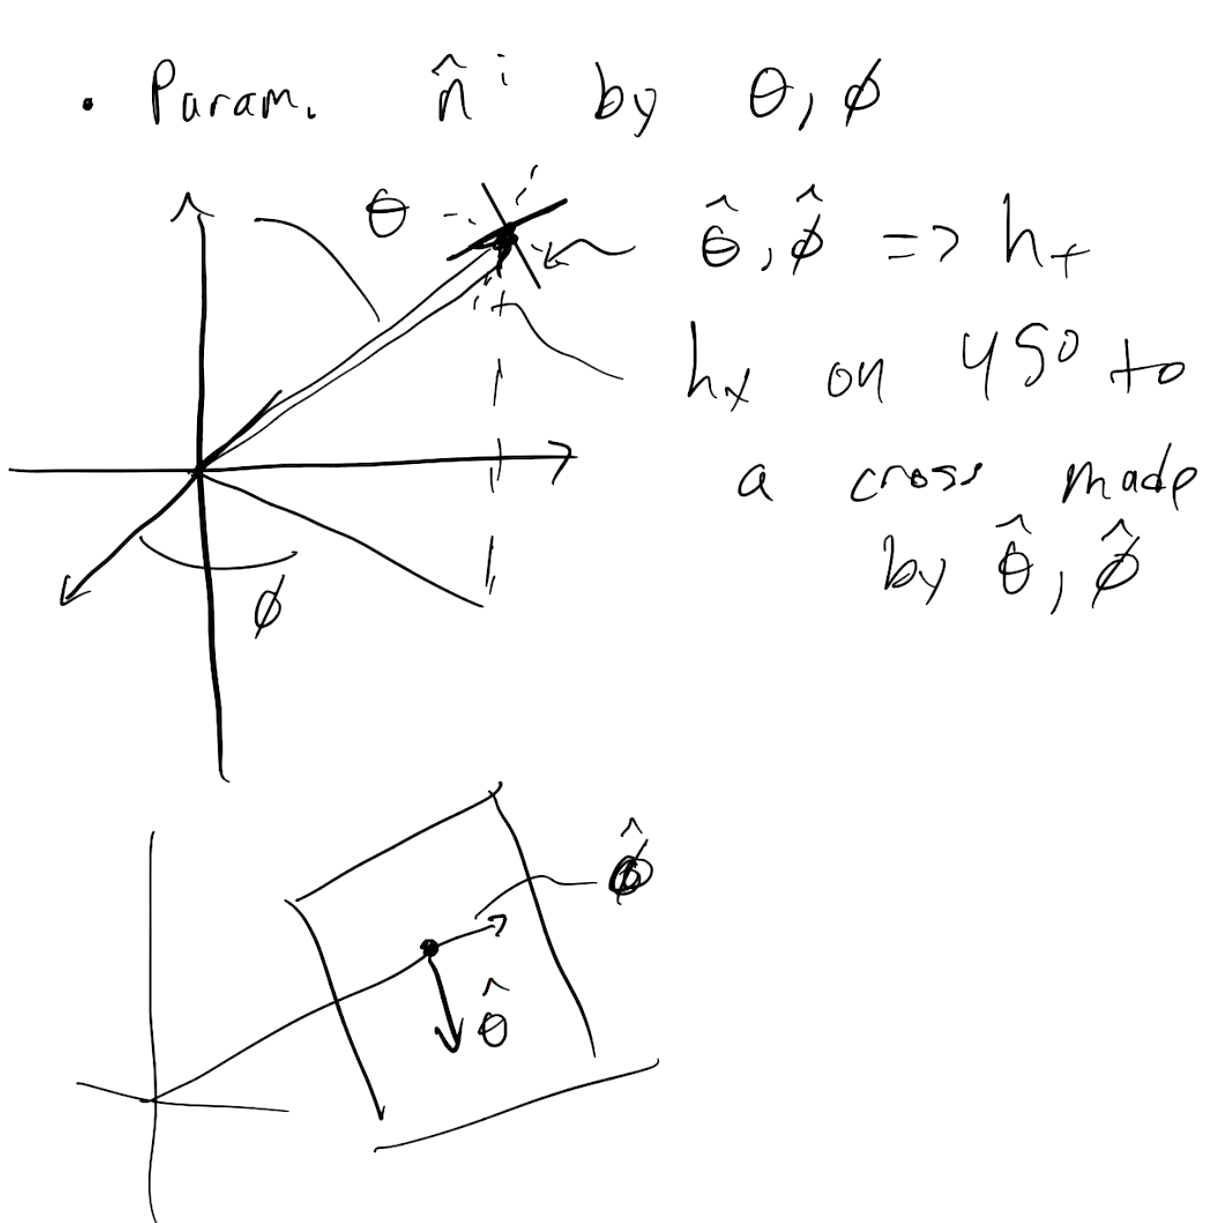
\includegraphics{figures/tt_projection_diagram.png}
    \caption{Schematic of TT-Projection operator}
    \label{fig:tt_projection}
\end{figure}


$$
h_+ = -2 (1+\cos ^2 \theta ) \frac{\mu}{r} (m \Omega)^{2/3} \cos(2 \Omega t_r - 2 \phi)
$$

$$
h_\times = -4 \cos \theta \frac{\mu}{r} (m \Omega)^{2/3} \sin(2 \Omega t_r - 2 \phi)
$$

\begin{remark}
Notice how $\Omega t_r - \phi$ comes in combinations. Also notice how the frequency of the waves are twice the orbital frequency: $2\Omega = \Omega_{GW}$. This is because the quadrupole moment is symmetric across a plane that intersects the center of mass of the system. Any asymmetry across this plane appears in the octopole moment and beyond.
\end{remark}

\begin{figure}
    \centering
    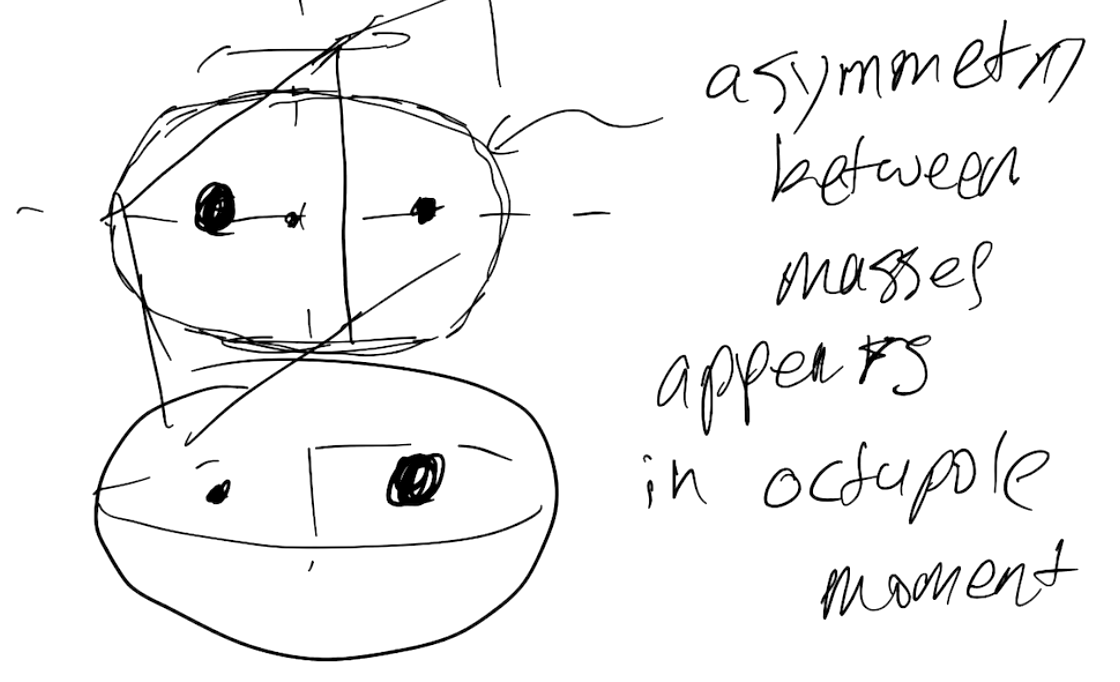
\includegraphics{figures/asymmetry_in_orbit.png}
    \caption{Asymmetry in the orbit of this binary appears in higher order moments only.}
    \label{fig:asymmetry}
\end{figure}

\section{Energy emitted from a binary}
In this section we will look into how to define the energy emitted from a gravitational wave system. Whether gravitational waves are an actual physical phenomena was a subtle problem that confused physicists for a while. The spring thought experiment shows us that energy can be delivered to a spring if it is damped, suggesting that this is indeed a physical process. Lets take a look.

Previously, we took our perturbed flat space metric and calculated the Ricci tensor to first order. To pin down the notion of energy, we will need to calculate the Ricci tensor to second order.
$$
R_{\mu \nu} = R_{\mu \nu}^{(0)} + R_{\mu \nu}^{(1)}
$$

The (0)th order term  = 0 because this is a solution to the vacuum Einstein equations. $R_{\mu \nu}^{(1)}$ and $R_{\mu \nu}^{(2)}$ can be found in Carroll Eq 7.153. The second order is quadratic in derivatives of the metric which suggests we need to perturb our metric to second order.

$$
g_{\mu \nu} = \eta_{\mu \nu} + h_{\mu \nu}^{(1)} + h_{\mu \nu}^{(2)}
$$

We then can get the second order Einstein equations that need to be solved:

$$
t_{\mu \nu} = - \frac{1}{8 \pi}  G_{\mu \nu}^{(2)}[h_{\alpha \beta}^{(1)}]
$$

$$
G_{\mu \nu}^{(1)}[h_{\alpha \beta}^{(2)}] = 8 \pi t_{\mu \nu}
$$

\begin{remark}
We would like this source term to obey the following physical properties motivated by electromagnetism:
\begin{itemize}
    \item quadratic in $h_{\mu \nu}^{(1)}$
    \item symmetric
    \item conserved: $\partial^\mu t_{\mu \nu} = 0$
\end{itemize}

\end{remark}

Although this is a nice interpretation, there is no local notion of gravitational energy in relativity. This is of course a drawback of the previous interpretation. There is no unique notion that satisfies a notion of gravitational energy, and this means that $t_{\mu \nu}$ is not unique. A famous example of this is the Landau-Lifshitz pseduo-tensor has the same properties as the source we defined previously. The final drawback is that $t_{\mu \nu}$ is not a gauge invariant quantity, which you can check.

Next time, we will look at the ideas presented first in Isaacson (1968), which introduces the two length scale approach with averaging.

Stay tuned!
\end{document}
